
\section{Conclusão}
\begin{frame}[fragile]
\begin{center}

  {\Large Como vocês construiriam esse sistema?}

  \vspace{2em}
  \pause

  {\Large Por que pares?}

  \vspace{2em}
  \pause

  \texttt{cons}, \texttt{car}, \texttt{cdr}

  \vspace{2em}
  \pause

  \textit{It is better to have 100 functions operate on one data structure than 10 functions on 10 data structures.} \\
  --- Alan Jay Perlis
\end{center}
\end{frame}

\begin{frame}
  Inteiros, racionais, reais e complexos
  \pause
  \begin{figure}
    \centering
    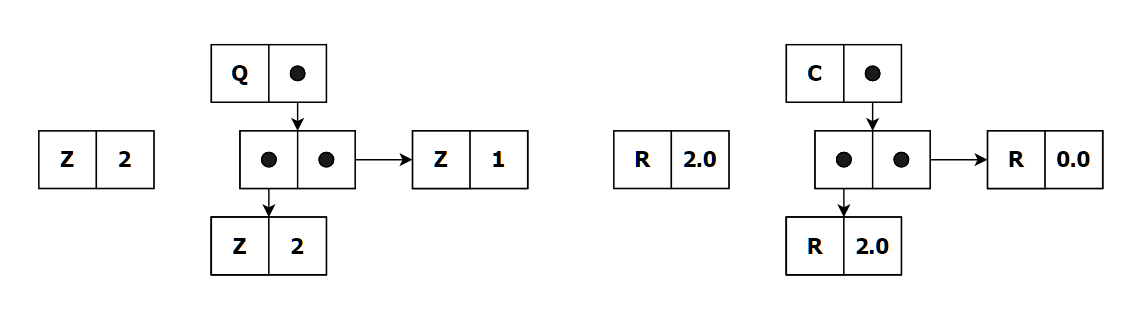
\includegraphics[width=0.8\linewidth]{z-q-r-c.png}
  \end{figure}
  \pause
  Polinômios e matrizes
  \pause
  \begin{figure}
    \centering
    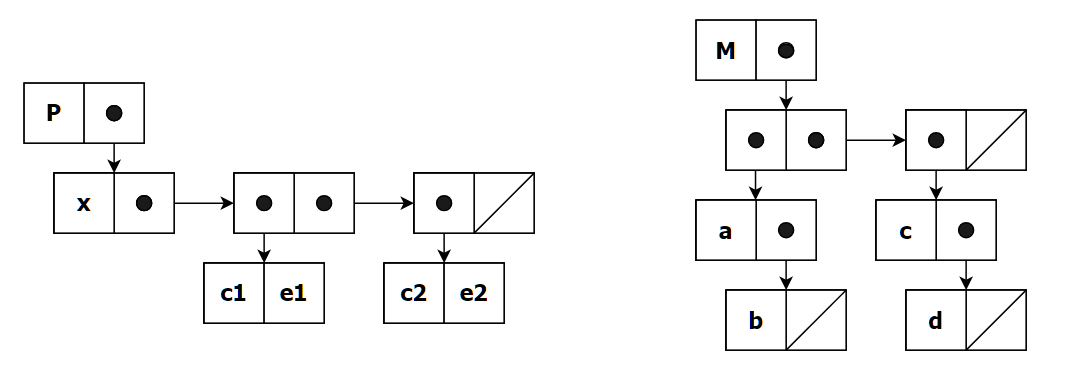
\includegraphics[width=0.8\linewidth]{matrix-and-poly.png}
  \end{figure}
\end{frame}



\begin{frame}
  \only<1>{
    \begin{figure}
      \centering
      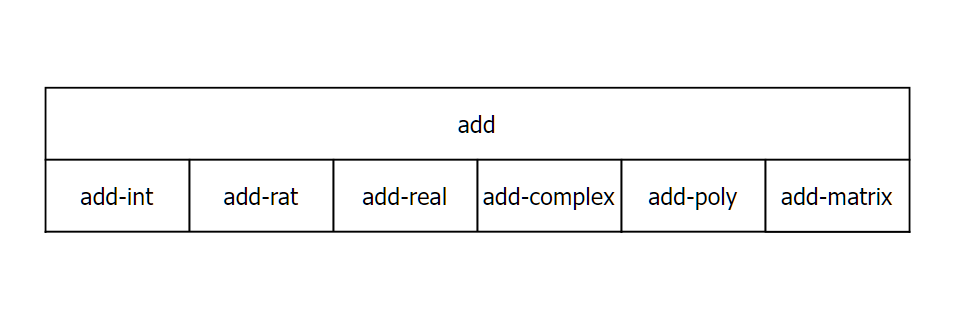
\includegraphics[width=1\linewidth]{defaddcomplete.png}
    \end{figure}
  }
  \only<2>{
    \begin{figure}
      \centering
      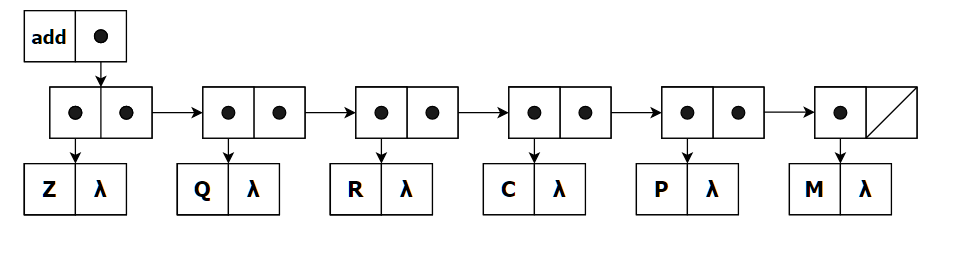
\includegraphics[width=0.85\linewidth]{add-real-def.png}
    \end{figure}
  }
\end{frame}

\begin{frame}
  \begin{center}

  Poderíamos sim ter utilizado tabelas hash para a construção desse sistema!

  \pause
  \vspace{2em}

  Maior eficiência

  \pause
  \vspace{2em}

  Manipulação menos simples do que pares! (\texttt{cons}, \texttt{car} e \texttt{cdr})

  \pause
  \vspace{2em}

  Por que Lua não usa pares, mas sim tabelas hash?
  \end{center}
\end{frame}